% Creating a simple Title Page in Beamer
\documentclass[xcolor={dvipsnames}, 10pt, brazil]{beamer}

% Pacotes
\usepackage{lipsum}
\usepackage{graphicx}
\usepackage{color}
\usepackage[table]{xcolor}
\usepackage{tikz}
\usepackage{tcolorbox}
\usepackage{amsmath}
\usepackage{amsfonts}
\usepackage{amssymb}
\usepackage{mathrsfs}
\usepackage{mathtools}
\usepackage{enumitem} 
\usepackage{float}
\usepackage[utf8]{inputenc}	
\usepackage[portuguese]{babel}
\usepackage{caption}

\usepackage{longtable}
\usepackage{wrapfig}
\usepackage{subfigure}

% Theme choice:
\usetheme{CambridgeUS}

% Cores personalizadas
\definecolor{PROFMATgreen}{RGB}{0, 138, 163}
\definecolor{UFTgreen}{RGB}{0, 137, 124}
\definecolor{UFTblue}{RGB}{0, 84, 132}
\definecolor{UFTyellow}{RGB}{253, 185, 46}
\definecolor{UFTgray}{RGB}{132, 134, 136} 
% Ativar numeração de tabelas
\setbeamertemplate{caption}[numbered]

% Definir novo estilo de item com quadrado verde
\setlist[itemize,1]{label=\textcolor{UFTgreen}{\rule{1ex}{1ex}}}

\setbeamercolor*{structure}{bg=UFTgreen,fg=black}

\setbeamercolor*{palette primary}{fg=black,bg=PROFMATgreen}
\setbeamercolor*{palette secondary}{fg=white,bg=UFTblue}
\setbeamercolor*{palette tertiary}{fg=black,bg=UFTgreen}
\setbeamercolor*{palette quaternary}{fg=white,bg=black}

\setbeamercolor{section in toc}{fg=black,bg=white}
\setbeamercolor{alerted text}{fg=white}

\setbeamercolor*{item}{fg=PROFMATgreen}

\setbeamercolor{block title}{bg=UFTgreen,fg=white}
\setbeamercolor{block body}{bg=UFTgray!10,fg=black}

\setbeamercolor{titlelike}{fg=white, bg=UFTblue}
\setbeamercolor{frametitle}{bg=UFTgray!20,fg=UFTgreen}



\setbeamertemplate{background}{
    \parbox[c][\paperheight][c]{\paperwidth}{
        \vfill
        
\includegraphics[width=\paperwidth,height=\paperheight,keepaspectratio]{img/modelo/bakcground.png} 
        \vfill
    }
}


% Customizar a página de título
\setbeamertemplate{title page}{
    \vbox{}
\begin{minipage}{0.3\linewidth}
        \centering
        
\includegraphics[width=4cm]{img/logo-icmc.png}
    \end{minipage}
    \hfill
    \begin{minipage}{0.3\linewidth}
        \centering
        
\includegraphics[width=3.5cm]{img/logo-lot-azul.png}
    \end{minipage}
    
    %\vfill
    \vskip1em\par
    \begingroup
        \centering
        \begin{beamercolorbox}[sep=8pt,center,shadow=true,rounded=false]{title}
            \usebeamerfont{title}\inserttitle\par%
            \ifx\insertsubtitle\@empty%
            \else%
                \vskip0.25em%
                {\usebeamerfont{subtitle}\usebeamercolor[fg]{subtitle}\insertsubtitle\par}%
            \fi%
        \end{beamercolorbox}%
        \vskip1em\par
        \begin{beamercolorbox}[sep=6pt,center]{author}
            \usebeamerfont{author}\insertauthor
        \end{beamercolorbox}
        \vskip0.2em\par
        \begin{beamercolorbox}[sep=5pt,center]{advisor}
            \usebeamerfont{institute} \advisorname
        \end{beamercolorbox}
        \vskip0.2em\par
        \begin{beamercolorbox}[sep=5pt,center]{institute}
            \usebeamerfont{institute}\insertinstitute
        \end{beamercolorbox}
        \vskip0.2em\par
        \begin{beamercolorbox}[sep=5pt,center]{date}
            \usebeamerfont{institute}\insertdate
        \end{beamercolorbox}
        \vskip0.5em\par
    \endgroup
    \vfill
}


% Remover bordas arredondadas dos blocks
\makeatletter
\setbeamertemplate{blocks}[default] % Isso remove o arredondamento
\makeatother


% Pacotes de citações
% ---

\usepackage[alf,abnt-etal-text=it,abnt-repeated-author-omit=yes,abnt-etal-list=0,abnt-etal-cite=3,abnt-emphasize=bf]{abntex2cite}	% Citações padrão ABNT



\setbeamercolor{bibliography entry author}{fg=black}
\setbeamertemplate{bibliography item}{\newblock}


\setbeamertemplate{frametitle continuation}{}

% Redefinir o separador para um traço
% Redefinir o separador
\captionsetup[figure]{labelformat=simple, labelsep=endash, textformat=period, font=footnotesize}
\captionsetup[table]{labelformat=simple, labelsep=endash, textformat=period, font=footnotesize}


% Redefine espaçamento antes e depois da legenda em figuras e tabelas
\captionsetup[figure]{aboveskip=2pt, belowskip=0pt}
\captionsetup[table]{aboveskip=2pt, belowskip=0pt}


% Define uma penalidade alta para a hifenização
\hyphenpenalty=10000
\tolerance=10000


% Personalizando o estilo da tabela de conteúdos
\setbeamertemplate{section in toc}[sections numbered]
\renewcommand{\thesection}{\textcolor{PROFMATgreen}{\arabic{section}}}
\renewcommand{\thesubsection}{\textcolor{PROFMATgreen}{\arabic{section}.\arabic{subsection}}}

\setbeamersize{text margin left=0.8cm, text margin right=0.8cm}

% Informações do documento
\title[Otimização em Alocação Multiclínica]{Técnicas de Otimização na Alocação de Médicos em Unidades de Diagnóstico por Imagem}
% \subtitle{Subtítulo Opcional}
\author[Thiago Mariotti]{Thiago Rafael Mariotti Claudio}
\institute[USP]{Universidade de São Paulo}
\date{24 de junho de 2026}

% Definir o nome do orientador
\newcommand{\advisorname}{\textbf{Orientadora:}  Profª. Drª. Maristela Oliveira dos Santos}

\begin{document}

% Slide (frame) de título
\begin{frame}
    \titlepage
\end{frame}


% Sumário
\begin{frame}[t]
    \frametitle{Sumário}
    \tableofcontents
\end{frame}

% =====================================================================
% §1 INTRODUÇÃO
% Arco: contexto/relevância -> escassez/impacto -> problema real ->
%       objetivos + virada mono->bi-objetivo (pivô vs. qualificação)
% =====================================================================
\section{Introdução}

%%% Frame 1.1 — Hook: o setor em números
\begin{frame}{O setor de diagnóstico por imagem em números}

    \begin{block}{Relevância clínica e econômica}
        \begin{itemize}
            \item 2,4 bilhões de exames diagnósticos realizados anualmente \cite{MedicinaSA2024}.
            \item Receita bruta de R\$ 24 bilhões movimentada em 2022 \cite{Abramed_2023}.
            \item Diagnóstico precoce $\rightarrow$ melhor acompanhamento, menor custo relativo \cite{OBRIEN_2007,Yasui_Fujiwara_Okitsu_Yonemitsu_Ito_Yokosuka_2012}.
        \end{itemize}
    \end{block}

    % TODO: falar 30s sobre a escala do setor como gancho.
    \vspace{2.5cm}
\end{frame}

%%% Frame 1.2 — Escassez + impacto operacional
\begin{frame}{Escassez de profissionais e impacto operacional}

    \begingroup
    \setbeamercolor{block title}{fg=white, bg=red!40}
    \setbeamercolor{block body}{bg=red!10}
    \begin{block}{Gargalo de mão de obra especializada \cite{Liebel_Dias_Schneider_SaScielo2021,RSNA_2024}}
        \begin{itemize}
            \item Crescimento estimado de 6\% para 18\% em vagas não preenchidas.
            \item Brasil: $\approx$ 1,51 mil médicos para cada 1,99 milhão de habitantes (2017).
            \item Equipamentos ociosos, filas e pressão sobre margens operacionais \cite{ANS_2024}.
        \end{itemize}
    \end{block}
    \endgroup

    % TODO: conectar escassez -> necessidade de escalas otimizadas.
    \vspace{2cm}
\end{frame}

%%% Frame 1.3 — O problema abordado
\begin{frame}{O problema abordado}

    \begingroup
    \setbeamercolor{block title}{fg=white, bg=orange!40}
    \setbeamercolor{block body}{bg=orange!10}
    \begin{block}{Escalonamento médico em rede de clínicas}
        \begin{itemize}
            \item Múltiplas unidades \textbf{autônomas} que compartilham profissionais.
            \item Escalas feitas \textbf{manualmente} pelo setor de operações: lento, sem garantia de otimalidade.
            \item Relação \textit{vários-para-vários} médico--unidade $\rightarrow$ explosão combinatória.
        \end{itemize}
    \end{block}
    \endgroup

    \begingroup
    \setbeamercolor{block title}{fg=white, bg=cyan!40}
    \setbeamercolor{block body}{bg=cyan!10}
    \begin{block}{Proposta}
        Gerar escalas otimizadas: maximizar atendimento com a equipe existente \emph{e} minimizar remanejamentos entre unidades \cite{Rousseau_Pesant_Gendreau_2002,Robinson_Chen_2003}.
    \end{block}
    \endgroup
\end{frame}

%%% Frame 1.4 — Objetivos + virada mono->bi-objetivo
\begin{frame}{Objetivos da pesquisa}

    \begin{block}{}
        \begin{itemize}
            \item Modelagem matemática do escalonamento médico em múltiplas unidades.
            \item Investigação \textbf{bi-objetivo}: exames não atendidos \emph{vs.} trocas de clínica.
            \item Avaliar três famílias de solução: exata, MIP-heurísticas e meta-heurística.
            \item Contribuir para a literatura de escalonamento médico multiunidade.
        \end{itemize}
    \end{block}

    \begingroup
    \setbeamercolor{block title}{fg=white, bg=UFTblue}
    \setbeamercolor{block body}{bg=UFTblue!10}
    \begin{block}{Evolução desde a qualificação}
        De objetivos tratados isoladamente para uma formulação \textbf{bi-objetiva} resolvida por método $\varepsilon$-restrito.
    \end{block}
    \endgroup
    % TODO: enfatizar que esta é a mudança central do trabalho.
\end{frame}

\section{Definição do Problema}

%% Elaborar nesta seção a definição formal do problema, incluindo:
%% - Descrição do problema (priorizar ilustrações e exemplos)
%% - Variáveis de decisão
%% - Função objetivo
%% Sempre que possível, comparar com a literatura
%% Fonte: docs/refs/dissertacao_tex/2-textual/problema.tex
%% Arco: cenário/agenda -> hipóteses -> notação -> restrições R1-R6 -> Z1/Z2 -> gamma.

%%% Frame 2.1 — Contextualização (visual: exemplo de agenda)
\begin{frame}{Contextualização do problema}

    % \vspace{-1cm}
    \begin{center}
        Médicos $\rightarrow$ Clínicas $\rightarrow$ Demanda \\
        {\footnotesize \cite{Rousseau_Pesant_Gendreau_2002,Robinson_Chen_2003}.}
    \end{center}

    \begin{figure}
            \centering
            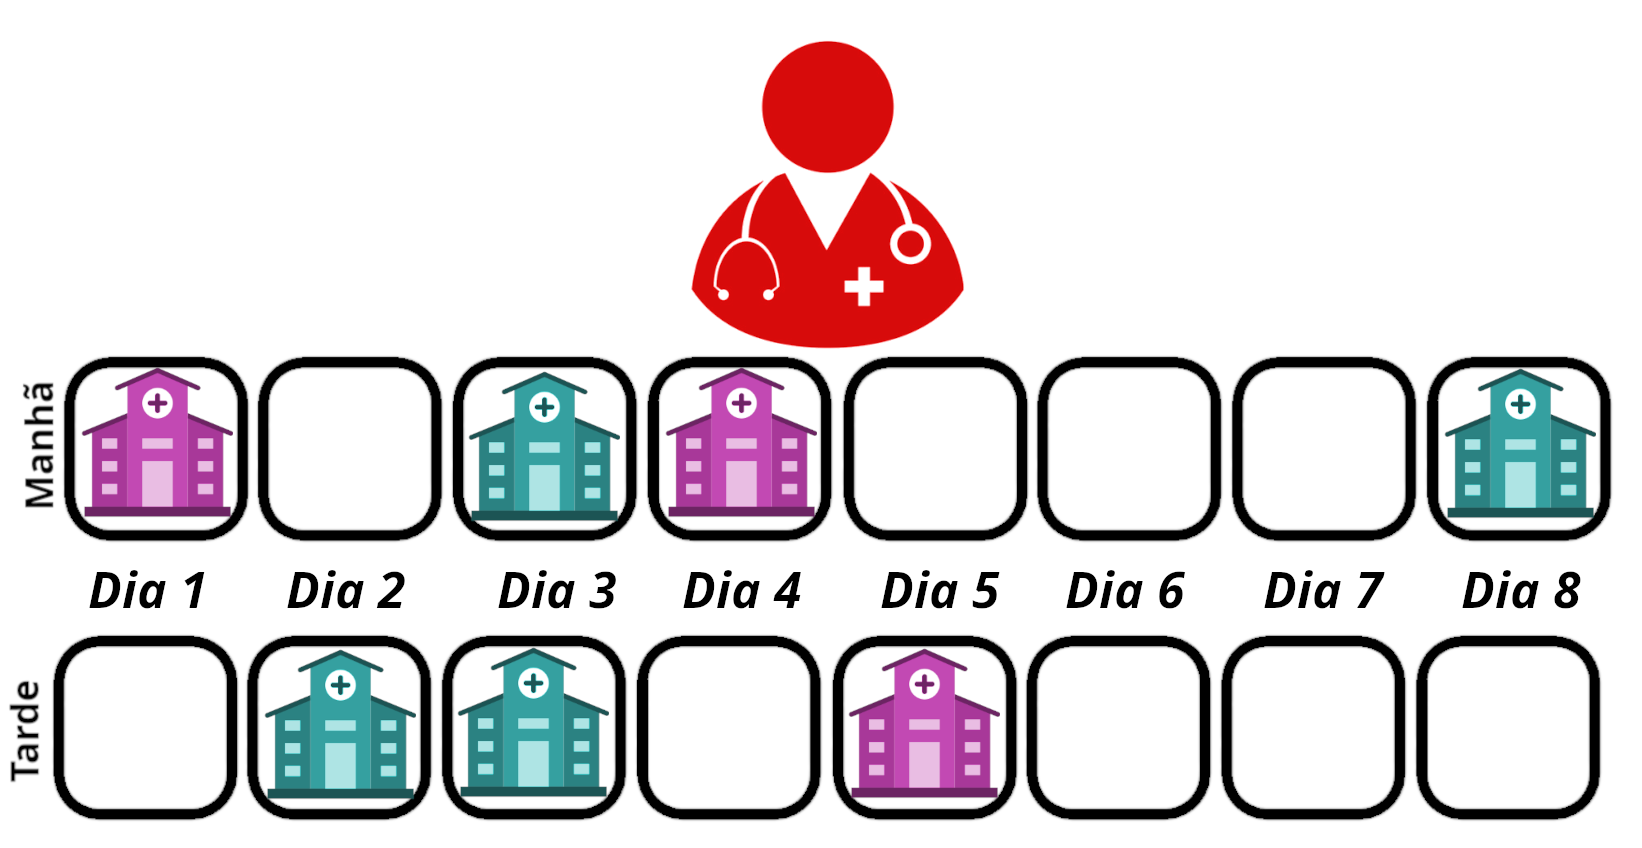
\includegraphics[width=0.6\linewidth]{img/exemplo-schedule-medico.png}
            \caption{Agenda de um médico ao longo do horizonte}
            \label{fig:ex-agenda}
        \end{figure}
    \end{frame}

    \vspace{-1cm}

    % \begin{center}
        
    % \end{center}

%%% Frame 2.2 — Hipóteses de modelagem (tabela)
\begin{frame}{Hipóteses de modelagem}
    \begin{footnotesize}
        \begin{table}
            \centering
            \begin{tabular}{cl}
                \toprule
                \textbf{Hipótese} & \textbf{Descrição} \\
                \midrule
                \textit{H1} & Todas as clínicas atendidas (ao menos cobertura mínima). \\
                \textit{H2} & Médico associado a uma única unidade por dia. \\
                \textit{H3} & Médico associado a uma sala da clínica. \\
                \textit{H4} & Médico realiza exames conforme a demanda da unidade. \\
                \textit{H5} & Atendimentos $-$ demanda $=$ exames não atendidos. \\
                \textit{H6} & Agenda irregular: sem limite de trocas entre clínicas. \\
                \textit{H7} & Condição inicial (histórico) $\rightarrow$ minimizar remanejamentos. \\
                \bottomrule
            \end{tabular}
        \end{table}
    \end{footnotesize}
    % TODO: H1 -> cobertura (R6); H2-H3 -> unicidade (R2-R3); H6-H7 -> trocas (Z2/gamma).
\end{frame}

%%% Frame 2.3 — Notação (conjuntos, parâmetros, variáveis)
\begin{frame}{Notação}
    \begin{small}
        \begin{columns}[T]
            \begin{column}{0.5\textwidth}
                \textbf{Índices e conjuntos}
                \begin{tabular}{ll}
                    $i \in I$ & Médicos \\
                    $u \in U$ & Unidades \\
                    $d \in D$ & Dias \\
                    $t \in T$ & Turnos \\
                    $U_i$     & Unidades de $i$ \\
                    $I_u$     & Médicos de $u$ \\
                \end{tabular}

                \vspace{0.4em}
                \textbf{Parâmetros}
                \begin{tabular}{ll}
                    $e_{udt}$ & Demanda de exames \\
                    $s_{udt}$ & Salas disponíveis \\
                    $q_{idt}$ & Capacidade do médico \\
                    $a_{idt}$ & Disponibilidade $(0/1)$ \\
                    $b_{udt}$ & Há demanda? $(0/1)$ \\
                \end{tabular}
            \end{column}
            \begin{column}{0.5\textwidth}
                \textbf{Variáveis de decisão}
                \begin{tabular}{ll}
                    $x_{iudt}$ & Aloca $i$ em $u$, dia $d$, turno $t$ \\
                    $w_{iud}$  & Aloca $i$ em $u$ no dia $d$ \\
                    $c_{udt}$  & Exames não atendidos \\
                    $z_{id}$   & $i$ trocou de clínica no dia $d$ \\
                \end{tabular}

                \vspace{0.8em}
                \begin{block}{Período}
                    Dia $d$ $\times$ turno $t$ (manhã/tarde); domingo com demanda $0$.
                \end{block}
            \end{column}
        \end{columns}
    \end{small}
\end{frame}

%%% Frame 2.4 — Restrições estruturais R1-R6 (+ chave visual)
\begin{frame}{Restrições estruturais}
    \resizebox{\textwidth}{!}{\begin{minipage}{1.25\textwidth}
        \begin{alignat}{2}
            \sum_{u \in U_i} x_{iudt} &\leq a_{idt} \quad && \forall i \in I, d \in D, t \in T \label{eq:r1} \\
            \sum_{u \in U_i} w_{iud} &\leq 1 \quad && \forall i \in I, d \in D \label{eq:r2} \\
            x_{iudt} &\leq w_{iud} \quad && \forall i \in I, u \in U, d \in D, t \in T \label{eq:r3} \\
            w_{iud} &= 0 \quad && \forall i \in I, u \notin U_i, d \in D \label{eq:r4} \\
            \sum_{i \in I_u} x_{iudt} &\leq s_{udt} \quad && \forall u \in U, d \in D, t \in T \label{eq:r5} \\
            \sum_{i \in I_u} x_{iudt} &\geq b_{udt} \quad && \forall u \in U, d \in D, t \in T \label{eq:r6} \\
            x_{iudt}, w_{iud} &\in \{0,1\} \quad && \forall i, u, d, t \label{eq:dom}
        \end{alignat}
    \end{minipage}}

    \vspace{0.3em}
    {\footnotesize\textbf{Chave:} (\ref{eq:r1})~disponibilidade, (\ref{eq:r2}--\ref{eq:r3})~uma unidade/dia, (\ref{eq:r4}--\ref{eq:r5})~elegibilidade e capacidade de salas, (\ref{eq:r6})~cobertura mínima.}
\end{frame}

%%% Frame 2.5 — Funções objetivo Z1 e Z2 (bi-objetivo)
\begin{frame}{Os "bi"-objetivos do problema}
    \begin{columns}[T]
        \begin{column}{0.54\textwidth}
            $Z_1$ --- \textbf{exames não atendidos} (operacional):
            \begin{alignat}{2}
                c_{udt} &\geq e_{udt} - \!\!\sum_{i \in I_u}\! q_{idt}\, x_{iudt} \label{eq:fo1-r1} \\
                \min\; & \sum_{u,d,t} c_{udt} \label{eq:fo1}
            \end{alignat}

            \vspace{0.5em}
            $Z_2$ --- \textbf{trocas de clínica} (ergonômico):
            \begin{equation}
                \min\; \sum_{i \in I}\sum_{d \in D} z_{id} \label{eq:fo2}
            \end{equation}
        \end{column}
        \begin{column}{0.46\textwidth}
            \begin{figure}
                \centering
                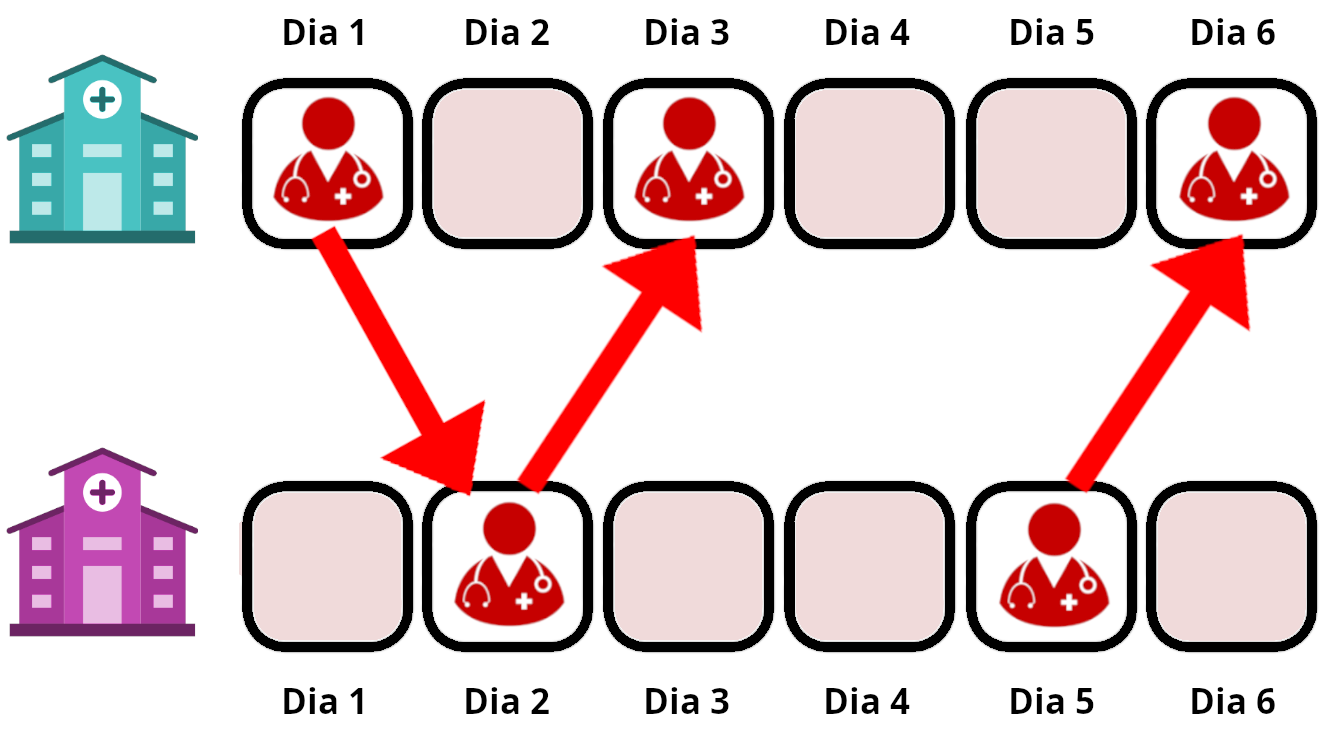
\includegraphics[width=\linewidth]{img/troca-examplo.png}
                \caption{Troca $=$ mudar de unidade entre dias.}
                \label{fig:ex-troca}
            \end{figure}
        \end{column}
    \end{columns}
    % TODO: objetivos conflitantes -> motiva fronteira de Pareto (Seção 3).
\end{frame}

%%% Frame 2.6 — Variável de estado gamma (contribuição de modelagem)
\begin{frame}{Detectando trocas}
    \begin{columns}[T]
        \begin{column}{0.55\textwidth}
            \begin{block}{Problema}
                Lacunas (dias sem trabalho) quebram a comparação ingênua de $w$ entre dias consecutivos.
            \end{block}
        \end{column}
        \begin{column}{0.5\textwidth}
            \resizebox{\linewidth}{!}{\begin{minipage}{1.15\linewidth}
                {\small
                \begin{alignat}{2}
                    \gamma_{iud} &\geq w_{iud} \label{eq:g-def} \\
                    \sum_{u \in U_i} \gamma_{iud} &= 1 \label{eq:g-sum} \\
                    z_{id} &\geq \gamma_{iud} + \!\!\sum_{u' \neq u}\! \gamma_{i,u',d-1} - 1 \label{eq:g-swap}
                \end{alignat}
                }
                {\centering\tiny $\gamma_{iud}$ adaptado do GLSP~\cite{Fleischmann_Meyr_1997}.\par}
            \end{minipage}}
        \end{column}
    \end{columns}
    \begin{center}
        \begin{figure}
            \centering
            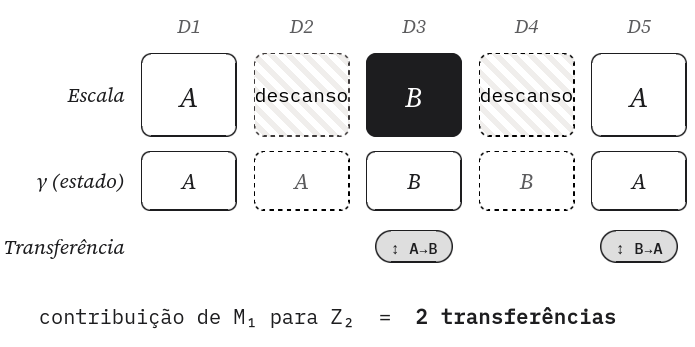
\includegraphics[width=0.7\linewidth]{img/04_nsga-05_gama.png}
            \caption{Estado $\gamma$ persiste nas lacunas.}
            \label{fig:gamma}
        \end{figure}
    \end{center}
\end{frame}

\section{Metodologia e Abordagens}

% Elaborar nesta seção a descrição das abordagens de solução, incluindo:
% 1. Método exato (MIP) para o problema bi-objetivo/eps-restrito
% 2. Heurísticas (construtivas e de melhoria) para o problema bi-objetivo/eps-restrito
% 3. Metaheurística NSGA-II para o problema bi-objetivo/eps-restrito, incluindo:
%    - Operadores mais impactantes
%    - Estratégia "Compacto" vs. "Expandido" para o encoding
% Fonte: docs/refs/dissertacao_tex/2-textual/heuristicas.tex
% Arco: eps-restrito -> MIP-heurísticas -> NSGA-II -> operadores -> encoding -> síntese.

%%% Frame 3.1 — Bi-objetivo + eps-restrito (TikZ Pareto)
\begin{frame}{Abordagem bi-objetiva: método \(\varepsilon\)-restrito}
    \begin{columns}[c]
        \begin{column}{0.54\textwidth}
            Objetivos conflitantes \(\rightarrow\) \textbf{fronteira de Pareto} \cite{Haimes_Wismer_1971}.
            \begin{itemize}
                \item \(Z_1\) como objetivo; \(Z_2 \leq \varepsilon\) como restrição.
                \item Limites por otimização lexicográfica.
                \item Grade de \textbf{7 pontos} \(\varepsilon\) por instância \cite{Saez-Aguado_Trandafir_2018}.
            \end{itemize}
        \end{column}
        \begin{column}{0.46\textwidth}
            \centering
            \begin{tikzpicture}[scale=0.82]
                \draw[->] (0,0) -- (4.3,0) node[right]{\footnotesize \(Z_1\)};
                \draw[->] (0,0) -- (0,3.5) node[above]{\footnotesize \(Z_2\)};
                \draw[very thick,UFTblue] (0.45,3.1) .. controls (1.1,0.95) and (2.1,0.65) .. (3.9,0.38);
                \foreach \y in {0.6,1.1,1.6,2.1,2.6} {\draw[dashed,UFTgray] (0,\y) -- (4.0,\y);}
                \foreach \p in {(0.6,2.6),(0.78,2.1),(1.12,1.6),(1.75,1.1),(3.05,0.6)}
                    {\fill[PROFMATgreen] \p circle (2.2pt);}
                \node[UFTgray] at (3.3,2.35){\tiny \(Z_2 \leq \varepsilon\)};
            \end{tikzpicture}
        \end{column}
    \end{columns}
    % TODO: grade compartilhada por todos os métodos MIP (comparabilidade ponto a ponto).
\end{frame}

%%% Frame 3.2 — MIP-heurísticas (TikZ janela deslizante)
\begin{frame}{MIP-heurísticas: decomposição temporal}
    \begin{center}
        \begin{tikzpicture}[scale=0.9]
            \foreach \i in {0,...,6} {
                \draw[fill=UFTgray!15] (\i,0) rectangle (\i+0.85,0.6);
            }
            \fill[UFTgreen!45] (2,0) rectangle (2.85,0.6);
            \fill[UFTgreen!45] (3,0) rectangle (3.85,0.6);
            \node[below] at (1.0,-0.05){\footnotesize fixado};
            \node[below] at (3.35,-0.05){\footnotesize janela \((d,t)\)};
            \node[below] at (5.7,-0.05){\footnotesize relaxado};
        \end{tikzpicture}
    \end{center}
    \vspace{0.4em}
    \begin{itemize}
        \item \textbf{Relax-and-Fix} (construtiva): resolve a janela, fixa \(w_{iud}\), avança.
        \item \textbf{Fix-and-Optimize} (melhoria): fixa fora da vizinhança, reotimiza.
        \item \textbf{Híbrido} RF~\(\rightarrow\)~FO: constrói e depois refina \cite{Turhan_Bilgen_2020}.
    \end{itemize}
\end{frame}

%%% Frame 3.3 — NSGA-II base (figura fluxo principal)
\begin{frame}{Meta-heurística: NSGA-II}
    \footnotesize
    Base evolutiva \cite{Deb_Pratap_Agarwal_Meyarivan_2002}:
    \begin{itemize} % TODO : itens lado a lado
        \item Ordenação não-dominada. \quad \item Distância de \textit{crowding}. \quad \item Elitismo (pais \(\cup\) filhos).
    \end{itemize}
    
    \begin{figure}
        \centering
        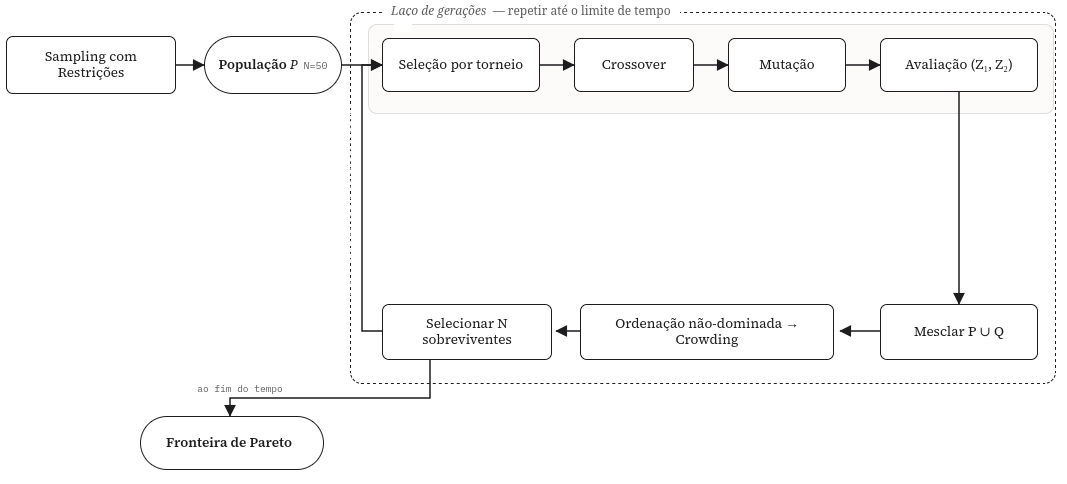
\includegraphics[width=\linewidth]{img/04_nsga-01_laco-principal.png}
        \caption{Fluxo principal do NSGA-II.}
        \label{fig:nsga-loop}
    \end{figure}
\end{frame}

%%% Frame 3.4 — Operadores customizados (2 figuras complementares)
\begin{frame}{Operadores customizados}
    Amostragem inicial \textbf{com consciência de restrições} \(+\) dois operadores que preservam a coerência temporal da agenda:
    \begin{columns}[T]
        \begin{column}{0.5\textwidth}
            \begin{figure}
                \centering
                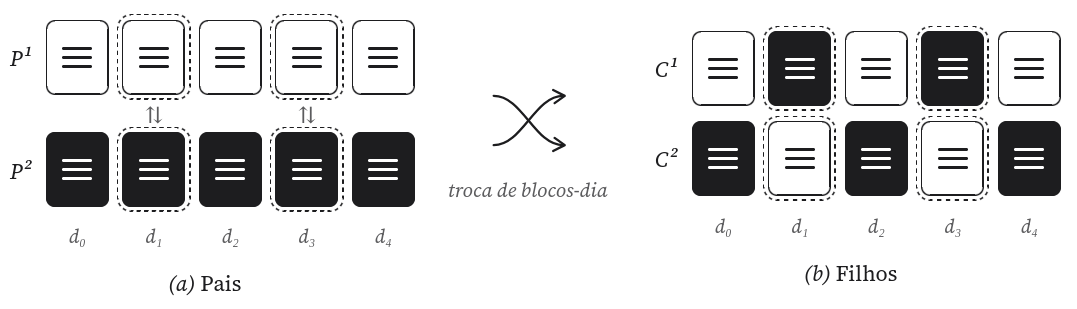
\includegraphics[width=\linewidth]{img/02_crossover.png}
                \caption{\footnotesize Cruzamento por blocos diários.}
            \end{figure}
        \end{column}
        \begin{column}{0.5\textwidth}
            \begin{figure}
                \centering
                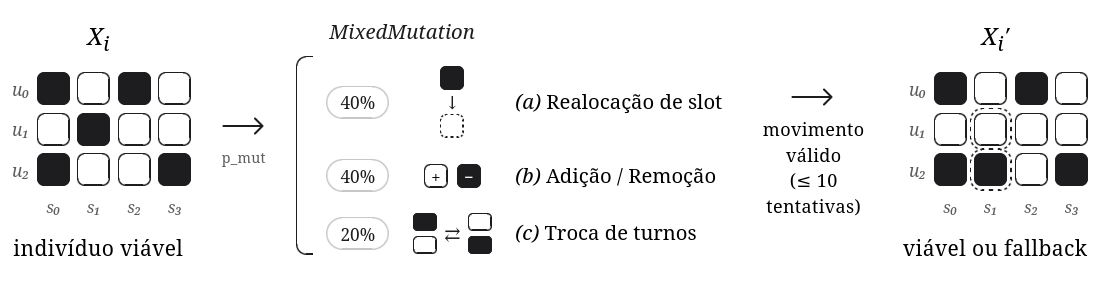
\includegraphics[width=\linewidth]{img/03_mutacao.png}
                \caption{\footnotesize Mutação por realocação de \textit{slot}.}
            \end{figure}
        \end{column}
    \end{columns}
\end{frame}

%%% Frame 3.5 — Encoding Compacto vs Estendido
\begin{frame}{Codificação: Estendido \emph{vs.} Compacto}
    \begin{figure}
        \centering
        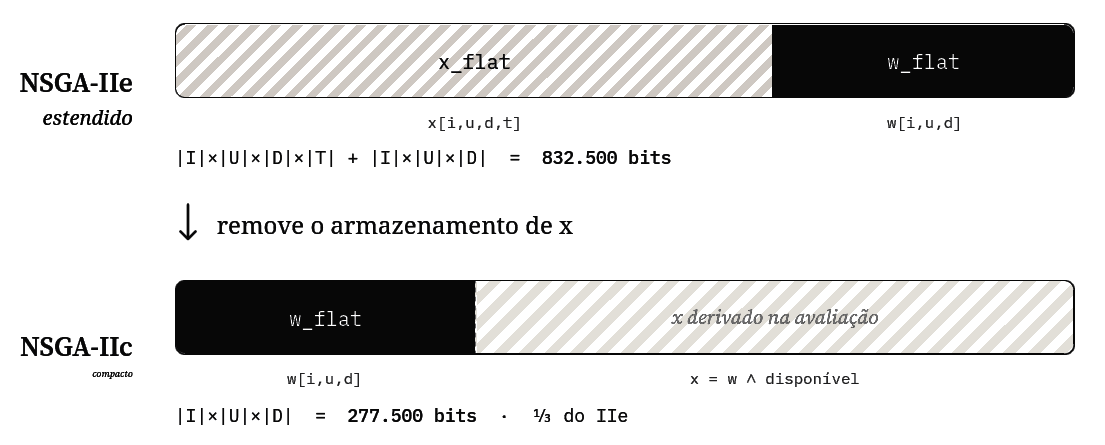
\includegraphics[width=0.82\linewidth]{img/05_encoding.png}
        \caption{Comparação dos \textit{encoders}.}
        \label{fig:encoding}
    \end{figure}
    \begin{itemize}
        \item \textbf{Estendido:} \(x_{iudt}\) e \(w_{iud}\) binários \(\rightarrow\) alta dimensionalidade.
        \item \textbf{Compacto:} gene por médico--dia (\(\approx w\)) \(\rightarrow\) \(\sim\)70\(\times\) menor, mais gerações.
    \end{itemize}
\end{frame}

%%% Frame 3.6 — Síntese das três famílias (transição p/ resultados)
\begin{frame}{Síntese: três famílias de solução}
    \begin{center}
        \begin{tabular}{lccc}
            \toprule
            & \textbf{Exato} & \textbf{MIP-heur.} & \textbf{NSGA-II} \\
            \midrule
            Garante factibilidade & sim & sim & parcial \\
            Escalabilidade (90 d) & baixa & média & alta \\
            Soluções por execução  & 7 (grade) & 7 (grade) & \(\sim\)100 \\
            \bottomrule
        \end{tabular}
    \end{center}
    \vspace{0.6em}
    \centering{\footnotesize Trade-offs distintos \(\rightarrow\) avaliados nos experimentos a seguir.}
\end{frame}

\section{Experimentos}

%% Elaborar nesta seção a descrição dos experimentos realizados, incluindo:
%% - Descrição do ambiente de teste (hardware, software, bibliotecas)
%% - Descrição das instâncias (exemplos, ilustrações, tabelas)
%% - Descrição dos experimentos (instâncias, parâmetros, métricas)
\section{Experimentos e Resultados}

% Desenvolver e discutir resultados obtidos (sem elaborar em detalhes de experimentos, que já foram descritos na seção anterior), incluindo:
% - Comparativos de resultados (parâmetros, instâncias, métricas) agrupados por métodos
% - Observações sobre a natureza multi-objetivo do problema e a influência da parametrização do $\varepsilon$-restrito
% - Comparativo cross-methods (MIP vs. heurísticas vs. metaheurísticas) com adendo a violçao da restrição no algoritmo genético (observa-se que os métodos não são diretamente comparáveis, mas é possível observar tendências, trade-offs e preparar perspectivas de trabalhos futuros)
% - Observações sobre a convergência do NSGA-II e a influência da parametrização

\section{Conclusões e Perspectivas}

% Pequena seção de conclusão e apanhados gerais, focando em:
% - Síntese dos resultados obtidos
% - Contribuições do trabalho
% - Limitações do estudo
% - Perspectivas de trabalhos futuros

% Seção de Referências
%\section{Referências}{}
% Slide da seção de Referências
\begin{frame}[t, allowframebreaks]

    \frametitle{Referências}

    \bibliography{references}
\end{frame}

\begin{frame}[t, allowframebreaks]

    \frametitle{Agradecimentos}


    \vspace{1cm}

    \begin{center}
    Agradeço aos órgãos \textbf{CNPq (164616/2024-1)} e \textbf{CAPES (88887.149213/2025-00)} pelo apoio financeiro para desenvolvimento da presente pesquisa.
    
    \vspace{0.5cm}

    \begin{minipage}[t]{0.475\textwidth}
        \begin{figure}
            \centering
            
\includegraphics[height=2.5cm]{img/capes-logo-transparente.png}
            %\caption{Agenda do médico}
            \label{fig:capes-logo}
        \end{figure}
    \end{minipage}
    \hfill
    \begin{minipage}[t]{0.475\textwidth}
        \begin{figure}
            \centering
            
\includegraphics[height=3cm]{img/cnpq-logo-transparente.png}
            %\caption{Ocupação de Salas}
            \label{fig:cnpq-logo}
        \end{figure}
    \end{minipage}
    
    \end{center}
    
\end{frame}

\begin{frame}
    \titlepage
\end{frame}

\end{document}